\chapter[Experimental Apparatus]{Experimental Apparatus\protect\footnote{This chapter is largely taken from Ref.~\cite{Thomassen2012} (the author's Master's Thesis).}}
\label{chap:Detector}

\section{The Large Hadron Collider}
The particle collisions analyzed in the present thesis were generated by the Large Hadron Collider (LHC) which is located $100\,\unit{m}$ underground in the French--Swiss border area at the outskirts of Geneva \cite{1748-0221-3-08-S08001}. Several pre-accelerators are employed in order to accelerate the protons to different energies and to split them into bunches, before they reach the LHC ring (see Fig.~\ref{fig:LHC}) to form two beams traveling in opposite directions. In this ring of $26.7\,\unit{km}$ circumference, 1232 superconducting dipole magnets are used to produce a magnetic field of up to $8.33\,\unit{T}$ in order to accelerate the protons to their final center of mass energy of $\sqrt{s} = 13\TeV$.
%\footnote{The maximum design energy is $14\TeV$. LHC has been operating with increasing energies over the years, and it is planned to reach the design goal in 2014?.}
Additionally, about 7000 magnets are used for trajectory corrections and bunch focusing. Once the final velocity is reached, the protons are directed onto each other at certain points around the accelerator ring, where they collide. The collision products, in general, are not stable, but decay to intermediate and final state particles which are detected by large detector devices such as ATLAS or CMS. The bunch spacing is such that interactions are separated in time by $25\,\unit{ns}$.\footnote{However, several interactions might occur at the same time when two bunches meet. This phenomenon is referred to as ``pile-up'' and must be corrected for at analysis time, mostly by means of geometrical separation of the primary interaction vertex and by subtraction of expected pile-up contributions.}

The design luminosity of LHC is $10^{34}\,\unit{cm^{-2}s^{-1}}$. The instantaneous luminosity is given by
\begin{eqnarray}
	L = \frac{N_p^2 n_b f_\text{rev} \gamma_r}{4\pi \epsilon_n \beta*} F
\end{eqnarray}
where $N_b$ is the number of particles per bunch, $n_b$ is the number of bunches per beam, $f_\text{rev}$ is the revolution frequency, $\gamma_r$ is the relativistic gamma factor, $\epsilon_n$ is the normalized transverse beam emittance, $\beta*$ is the beta function at the collision point, and $F$ is the geometric luminosity reduction factor due to the crossing angle at the interaction point.

\begin{figure}
	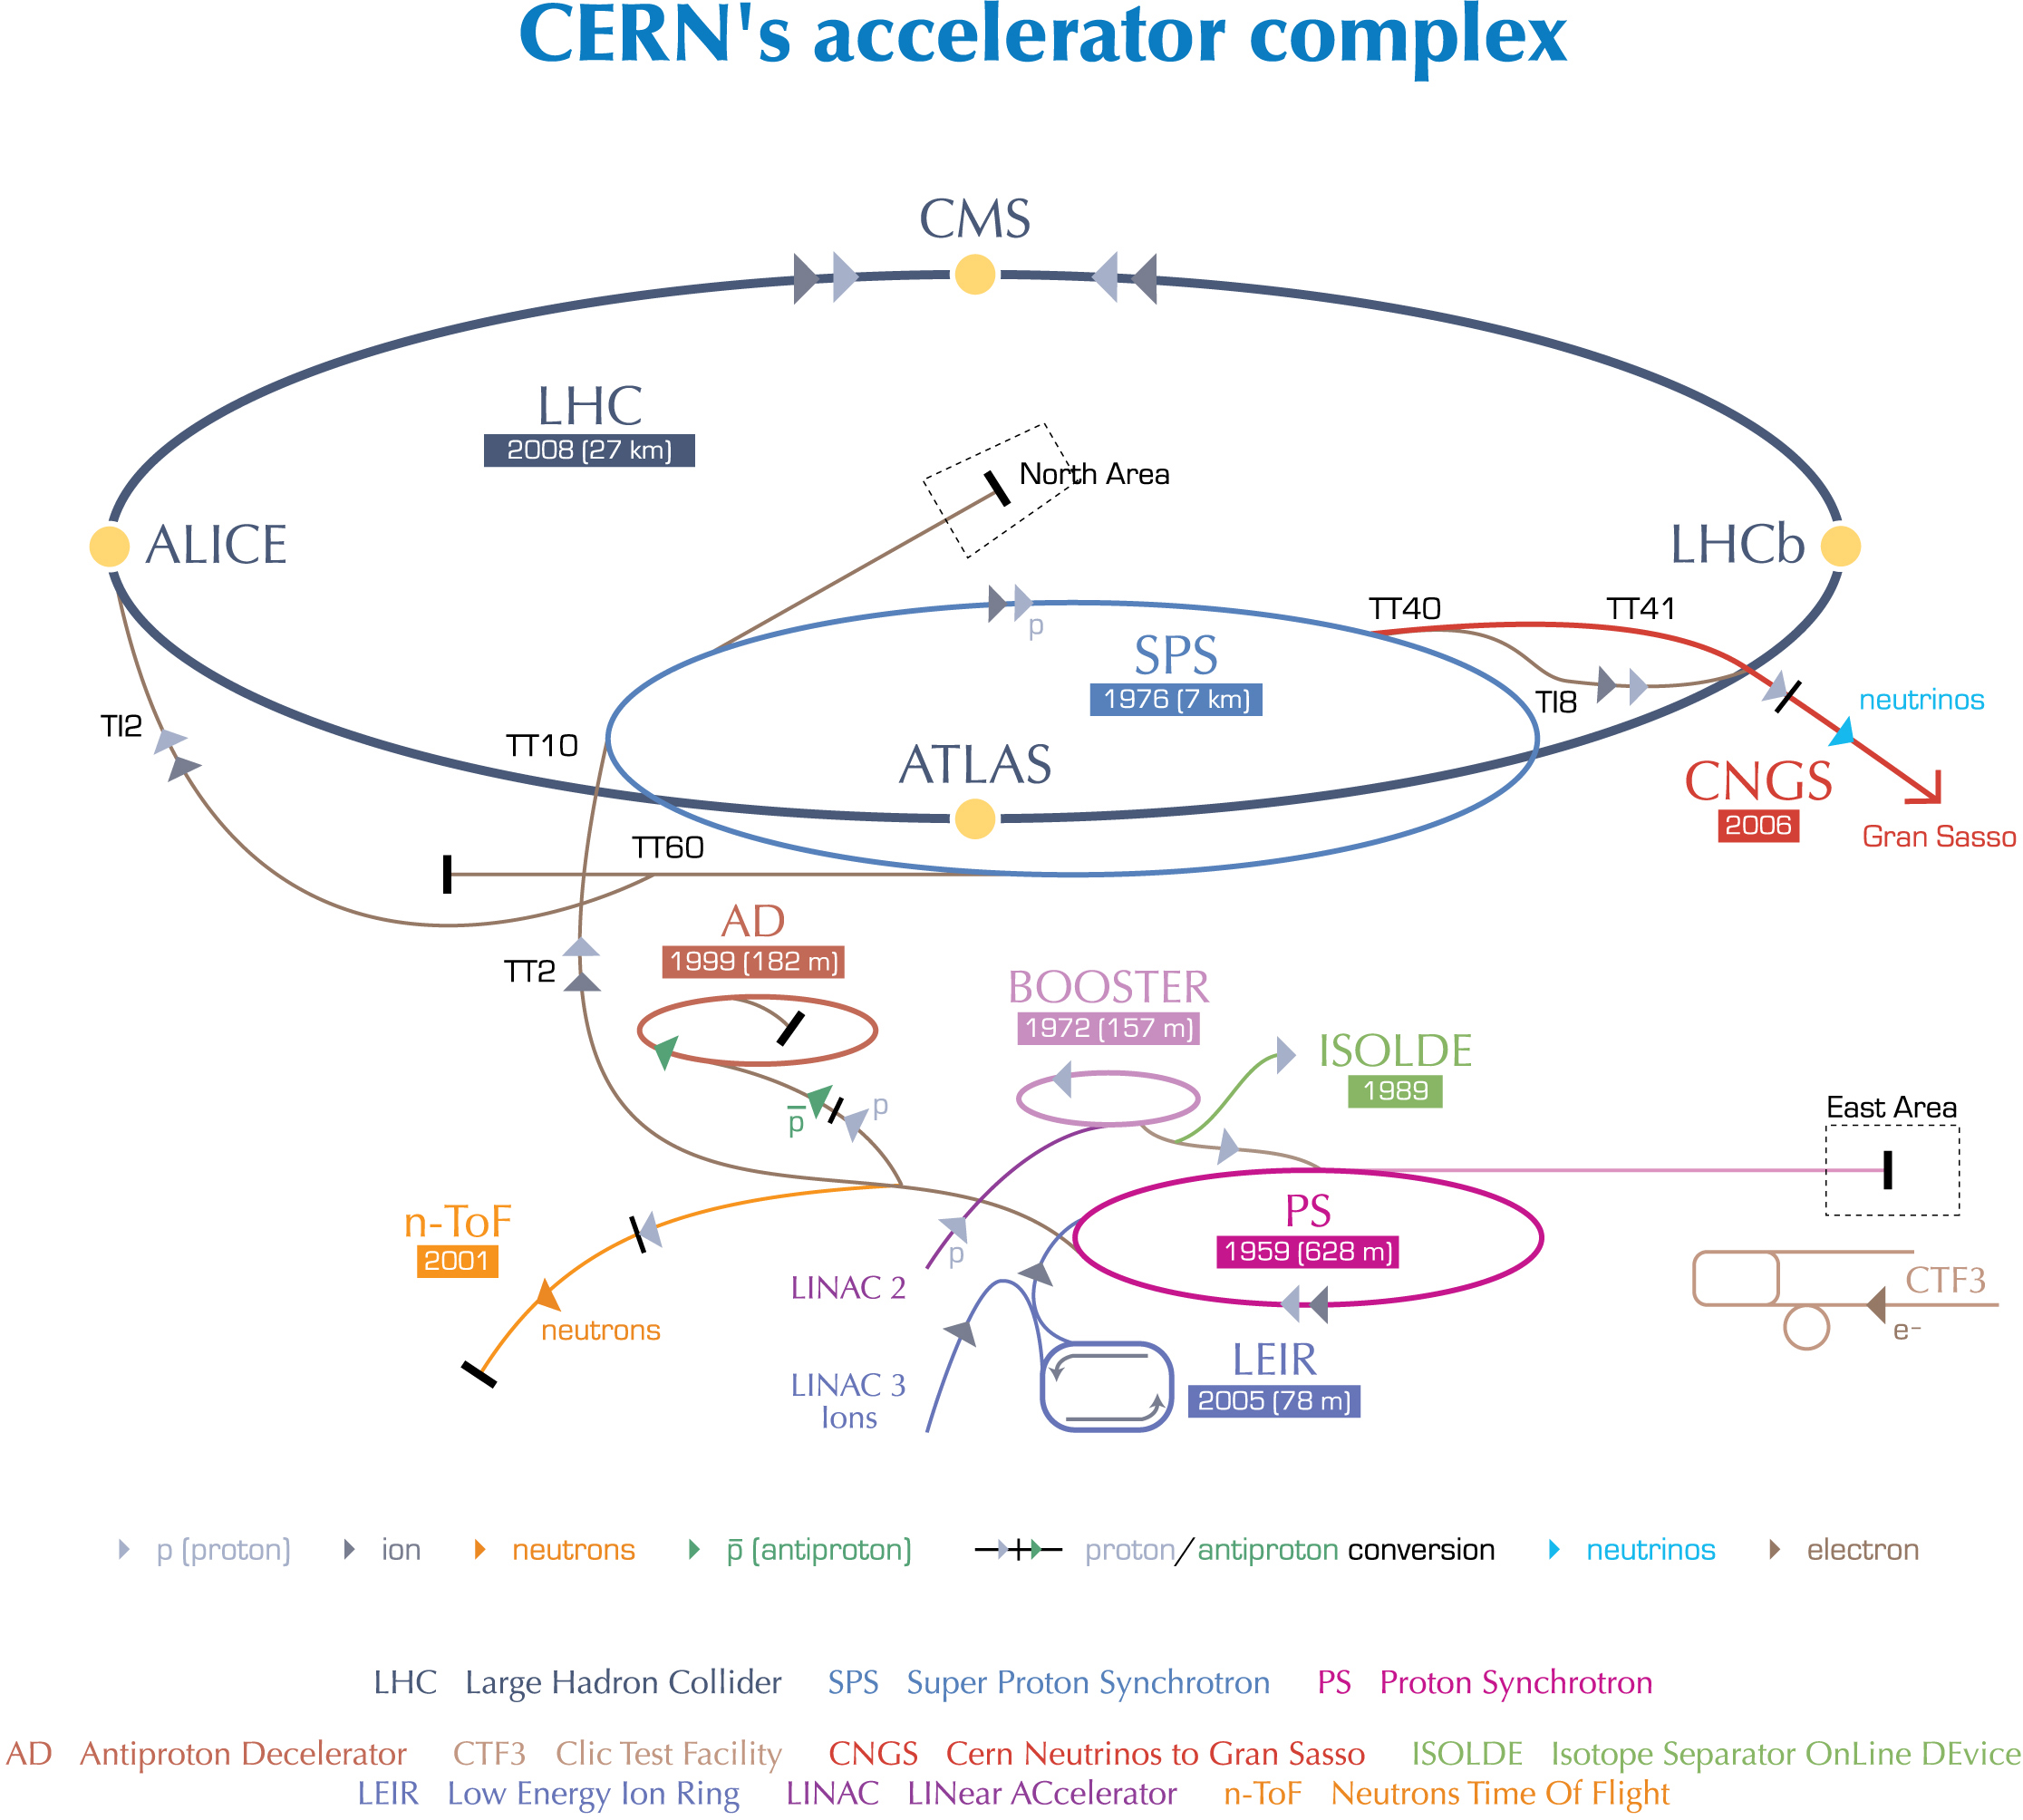
\includegraphics[width=.8\textwidth]{Detector/0812015}
	\centering
	\caption{CERN Accelerator Complex \cite{Christiane:1260465}. The diagram shows the different accelerators, detectors, and other facilities at CERN. For proton collisions, not all of the machinery is needed: Protons are initially accelerated to $50\MeV$ in a Linear Accelerator (LINAC~2). Then, they are transported to the Booster ($1.4\GeV$), to the Proton Synchrotron (PS, $25\GeV$) and the Super Proton Synchrotron (SPS, $450\GeV$) from where they are injected into LHC. The PS also takes care of arranging the protons in bunches with the correct spacing for LHC.}
	\label{fig:LHC}
\end{figure}

\section{The CMS Detector}
The Compact Muon Solenoid (CMS) is located at point 5 of the LHC accelerator ring and one of the two large, general purpose detector systems built at LHC. CMS consists of a large superconducting solenoid which contains a silicon-based tracker, an electromagnetic calorimeter made of scintillating lead-tungstate crystals, and a brass-based scintillating hadron calorimeter (see Fig.~\ref{fig:CMS}); the total weight is about 12500 tons \cite{Chatrchyan:2008zzk}. A special feature of CMS is its superconducting solenoid of $6\,\unit{m}$ internal diameter which creates a strong magnetic field ($3.8\,\unit{T}$) that is suitable for high precision measurements of charged particles at very high energies.

\begin{figure}
	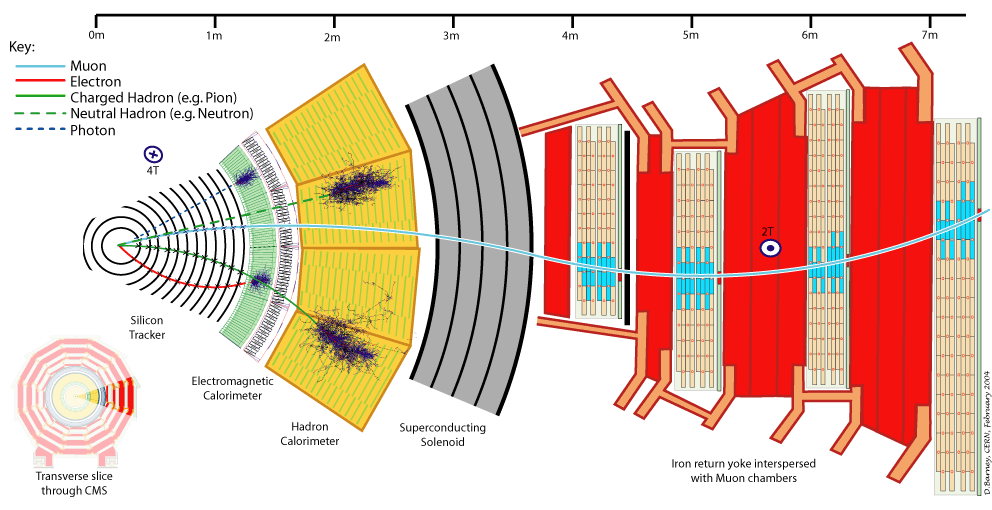
\includegraphics[width=\textwidth]{Detector/CMS_Slice}
	\centering
	\caption{A transverse slice through CMS \cite{CMSslice}. The illustration shows the most important detector components as well as examples of different particles as they are detected while traveling through the detector.}
	\label{fig:CMS}
\end{figure}

In order to describe the properties of particles observed in collision events, a coordinate system is defined. The origin is declared where the main interaction point is expected to occur. The $x$ axis points radially towards the center of the LHC, the $y$ axis points in the upward direction, and together with the $z$ axis that points along the beampipe (counterclockwise), a right-handed coordinate system is constructed. In cylindrical coordinates, the $z$ axis is the same, and $\phi$ is the azimuthal angle. Starting from the positive $z$ axis, the polar angle $\theta$ increases towards the center of the LHC. Since the polar angle $\theta$ is not Lorentz-invariant, the pseudorapidity $\eta$ is defined as a Lorentz-invariant alternative coordinate,\footnote{This quantity is the massless limit of the rapidity which is an additive measure of relativistic velocity and defined as $\log \frac{E + p_z}{E - p_z}$.}
\begin{eqnarray}
	\eta = - \log \tan \frac{\theta}{2}.
\end{eqnarray}
When the directional separation between particles needs to be determined,
\begin{eqnarray}
	\Delta R = \sqrt{(\Delta \eta)^2 + (\Delta \phi)^2}
\end{eqnarray}
comes in handy as a measure of two particles' separation in $\eta$ and $\phi$.

The following sections are concerned with the individual detector components used for the measurement of the particle properties that are recorded from collision events, along the lines of Ref.~\cite{Xie:1455454}.

\subsection{Tracking System}
In order to precisely reconstruct the path of charged particles in CMS, a tracking system based on silicon-based p--n junctions was installed. A high reverse-bias voltage is applied across the junction, creating a depletion zone with an electric field. When a charged particle passes this zone, it ionizes the silicon atoms, and the resulting electrons are free to move and create an electrical current which is detected. By setting up several layers containing a large number of such p--n junctions with small dimensions, a highly sensitive tracking device can be created. In total, 15400 tracking sensors are installed in CMS and operated at low temperature in order to minimzie the effects of radiation damage. The CMS tracking system consists of several parts:

\subsubsection*{Pixel Detector}
The Pixel Detector is located within $10\,\unit{cm}$ from the $z$ axis and is used to account for small displacements close to the primary vertex, To keep the occupancy per bunch crossing reasonably low, a pixel size of $100\,\mum \times 150\,\mum$ is used. The spatial resolution is $10\,\mum$ to $20\,\mum$.

\subsubsection*{Strip Detector}
The Strip Detectors are located both in the barrel as well as in the endcap regions of CMS. In either case, several layers of silicon strips are placed behind each other to provide similar functionality as in the case of the pixel detector. The dimensions are much wider than those of the pixels. In each detector region, they are chosen according to the corresponding production characteristics such that the occupancy will not be too high, so that a hit will provide informative value.

\subsection{Electromagnetic and Hadronic Calorimeter}
The calorimetry system is designed to measure the energies of incident particles. Depending on the particle type, the energy is deposited in different parts of the system \cite{Halkiadakis:2010mj}:

\begin{figure}
	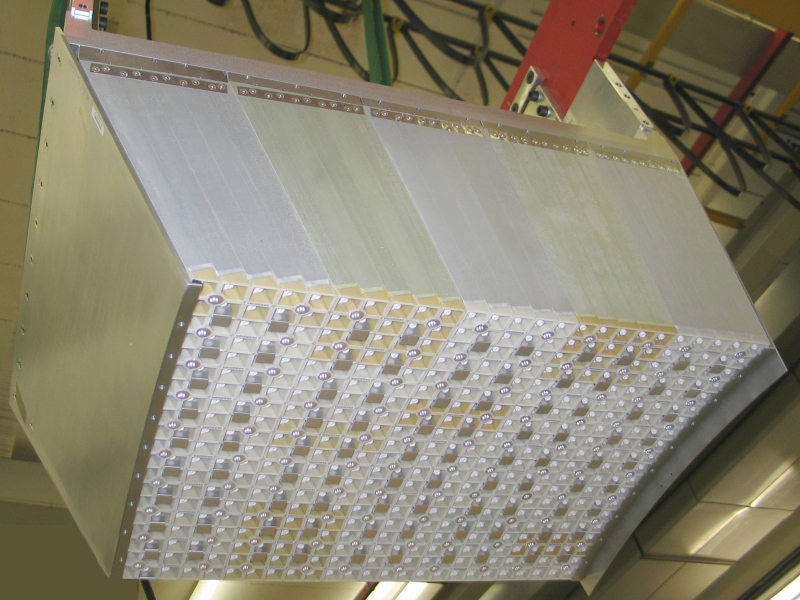
\includegraphics[width=.7\textwidth]{Detector/ECAL_crystal}
	\centering
	\caption{A module of the electromagnetic calorimeter consisting of 500 lead-tungstate crystals.}
	\label{fig:ECAL}
\end{figure}

\subsubsection*{Electromagnetic Calorimeter (ECAL)}
The task of the ECAL is to measure the energy of charged particles (especially electrons) and photons. The lead-tungstate (PbWO$_4$) material of the crystals is very dense, but optically transparent; a module is shown in Fig.~\ref{fig:ECAL}. When electrons or photons travel through, they lose energy in a cascade process due to bremsstrahlung and ionization (electrons) and $e^+ e^-$ pair production (photons). In addition, the crystals are excited so that they produce light from scintillation which is detected by photodetectors and used to infer the incident particle's energy.

In the barrel ($|\eta| \leq 1.479$), there are 61200 crystals with front face dimensions of $22\,\unit{mm} \times 22\,\unit{mm}$, covering 0.0174 in both $\eta$ and $\phi$, and a length of $230\,\unit{mm}$, corresponding to about 25 radiation lengths. In the endcap ($1.479 \leq |\eta| \leq 3.0$), there are 7324 crystals with a surface area of $28.6\,\unit{mm} \times 28.6\,\unit{mm}$ and a length of $220\,\unit{mm}$. An additional preshower detector is installed in front of the endcap component that helps distinguishing photons from neutral pions. This setup covers the $\eta$ range up to the forward region without any gaps.

\subsubsection*{Hadronic Calorimeter (HCAL)}
Like the ECAL, the HCAL is for the most part located inside the solenoid. While the ECAL is a homogeneous, the HCAL is a sampling calorimeter which means that it consists of alternating layers of an active, signal-generating medium, and a passive medium whose only purpose is to absorb energy. The active material is a plastic scintillator which is $3.7\,\unit{mm}$ thick and organized in a tile pattern. The scintillation light emitted in a certain $\eta$--$\phi$ cell is summed up optically, forming a ``tower'', collected by wavelength-shifting fibers, and channeled to hybride photodiodes.

The barrel part ($|\eta| \leq 1.4$) has 2304 towers, each covering 0.087 in $\eta$ and $\phi$. There are 15 absorption layers, mostly made from brass. To increase accuracy, a number of layers is placed at the outside of the magnet coil (Hadron Outer, HO). The endcap parts cover the region $1.3 \leq |\eta| \leq 3.0$ with 19 layers of active scintillating material, covering cell of width $5^\circ$ to $10^\circ$ in $\phi$ and 0.35 to 0.09 in $\eta$. In the very forward region ($3.0 \leq |\eta| \leq 5.0$), a fourth HCAL part (Hadron Forward, HF) consisting of an active quartz fiber medium and steel absorbers is located. The quartz fiber material emits Čerenkov light that is detected by photomultipliers with resolution 0.175 in $\eta$ and $10^\circ$ in $\phi$.

\subsection{Muon System}
The muon is about 200 times as heavy as the electron. Since the bremsstrahlung-induced dissipation in the calorimeter is proportional to $\text{mass}^{-2}$ \cite{bock2013particle}, it is suppressed by a factor of 40000. Therefore, muons can easily traverse the calorimeter system, so that other more specialized detector systems can be employed outside the calorimeter.

In the barrel, 250 drift tube (DT) chambers are used to identify muons. Four shells of stations are located at different distances from the $z$ axis, embedded in the return yoke of the solenoid (see Fig.~\ref{fig:muonSystem}). In the endcap, 468 cathode strip chambers (CSC) are arranged in concentric rings, most of them containing 36 CSCs. Charged particles travelling through the gas inside a CSC cause ionization, followed by a charged avalanche whose distribution is measured on the cathode plane. From this information, it is possible to reconstruct the track geometry. Each of the DT and CSC stations is accompanied by resistive plate chambers that are used for precise timing and velocity determination.

\begin{figure}
	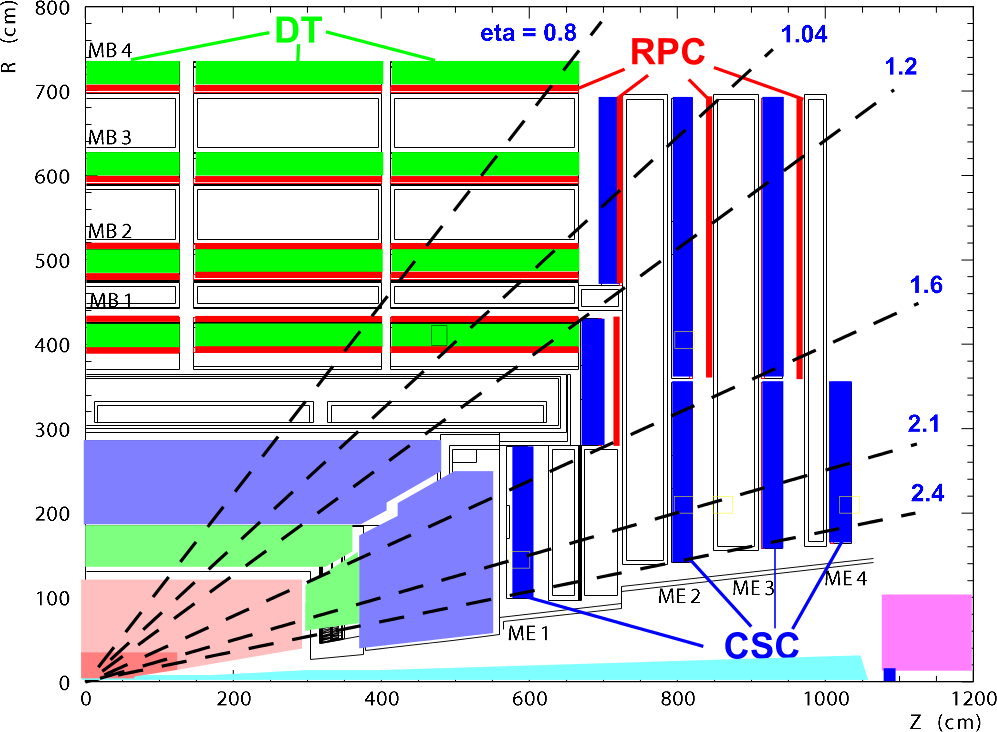
\includegraphics[width=\textwidth]{Detector/muon}
	\centering
	\caption{Sketch of the muon system in CMS in $r$--$z$ view. The drift tubes are displayed in dark-green, the cathode strip chambers in dark-blue, and the resistive plate chambers in dark-red. The light-colored areas are the tracker and calorimeter. The interaction point is located at the origin of the coordinate system.}
	\label{fig:muonSystem}
\end{figure}

\subsection{Trigger and Data Storage}
LHC performs about about $10^7$--$10^8$ proton--proton collisions per second. Since not all events can be stored (about $300\,\text{Hz}$), a rejection rate of about $10^5$ is required. First-level decisions are reached by the Level-1 (L1) trigger system which performs quick assessments of events within about 1\mus while the event data, about $0.5\,\text{MB}$ each, is held in buffers. Potentially interesting events are then forwarded to a dedicated computing farm where high-level triggers (HLT) run more precise reconstruction algorithms in order to decide which events should be kept.

Finally, accepted events are transmitted to the storage manager system which arranges the subsequent transfer to the permanent Tier-0 storage systems located at the CERN main site and at the Wigner Research Centre for Physics in Budapest (Hungary). From there, data is distributed to interested Tier-1 and Tier-2 sites across the globe for analysis purposes. Petabyte-range storage systems are employed world-wide to manage the large amounts of data that are used on a daily basis.
